\chapter{Experimental Data and Analysis Scripts}
\label{app:results_scripts}
This appendix provides the supplementary materials associated with the experimental campaigns detailed in Chapter~4. It collects the custom Python scripts developed to automate the two navigation pipelines---directed waypoint navigation and autonomous frontier-based exploration---to log the absolute Ground~Truth metrics, and to aggregate the statistical results across the multiple benchmarking iterations. For conciseness, only the methodologically relevant excerpt of each script is reported.

\section{Waypoint Sequence Definitions}
The three routes described in Section~\ref{subsec:wp-protocol} are defined as ordered lists of poses (position in the \texttt{map} frame, in metres, and heading in radians), loaded at run time by the driver node.

\begin{lstlisting}
# waypoints_hallway.yaml  --  Path A (Straight Corridor)
waypoints:
  - {x: 1.245, y:  1.620, yaw: -1.5708}   # WP0 (spawn)
  - {x: 1.245, y: -11.377, yaw: -1.5708}  # WP1 (goal)

# waypoints_angle.yaml  --  Path B (Sharp Corner)
waypoints:
  - {x:  0.0, y:  1.0, yaw: -1.5708}   # WP0 (spawn)
  - {x:  0.0, y: -0.5, yaw: -1.5708}   # WP1 (corner)
  - {x: -1.0, y: -0.5, yaw: -1.5708}   # WP2
  - {x: -1.3, y: -0.5, yaw: -1.5708}   # WP3 (goal)

# waypoints_obs.yaml  --  Path C (Cluttered Obstacle Course)
waypoints:
  - {x:  1.500, y: -3.000, yaw: -1.57}  # WP0 (spawn)
  - {x: -2.143, y: -3.631, yaw: -1.57}  # WP1
  - {x: -2.646, y: -5.523, yaw: -1.57}  # WP2
  - {x: -4.213, y: -8.274, yaw: -1.57}  # WP3
  - {x: -2.049, y: -8.099, yaw: -1.57}  # WP4 (near human model)
  - {x: -0.950, y: -7.990, yaw: -1.57}  # WP5 (near human model)
  - {x:  4.577, y: -8.276, yaw: -1.57}  # WP6
  - {x:  4.680, y: -7.201, yaw: -1.57}  # WP7
  - {x:  3.188, y: -4.613, yaw: -1.57}  # WP8
  - {x:  1.951, y: -2.987, yaw: -1.57}  # WP9
  - {x:  3.897, y: -2.086, yaw: -1.57}  # WP10 (goal)
\end{lstlisting}

\section{Waypoint Navigation Driver}
The driver node loads a sequence and dispatches it to Nav2 as a single \texttt{NavigateThroughPoses} goal, so that the robot flows through the intermediate poses without stopping. It also republishes the index of the currently active waypoint on \texttt{/current\_waypoint\_idx}, which the logger uses to segment the run. The clock is forced to simulated time, so that the reported durations are consistent with the rest of the stack.

\begin{lstlisting}[language=Python]
def make_pose(nav, x, y, yaw):
    pose = PoseStamped()
    pose.header.frame_id = 'map'
    pose.header.stamp = nav.get_clock().now().to_msg()   # sim-time (use_sim_time forced True)
    pose.pose.position.x = float(x)
    pose.pose.position.y = float(y)
    pose.pose.orientation.z = math.sin(yaw / 2.0)
    pose.pose.orientation.w = math.cos(yaw / 2.0)
    return pose

# Build the full pose list and dispatch a single continuous NavigateThroughPoses
# goal: the robot flows through the via-points without stopping at each one.
poses = [make_pose(nav, wp['x'], wp['y'], wp['yaw']) for wp in load_waypoints(path)]
current_idx = 0
idx_pub.publish(Int32(data=current_idx))        # active-waypoint index, for the GT logger
nav.goThroughPoses(poses)

while not nav.isTaskComplete():
    fb = nav.getFeedback()
    if fb and hasattr(fb, 'number_of_poses_remaining'):
        active_idx = len(poses) - fb.number_of_poses_remaining
        if active_idx != current_idx and active_idx < len(poses):
            current_idx = active_idx              # may skip a value for a fast base
            idx_pub.publish(Int32(data=current_idx))
    time.sleep(0.1)

idx_pub.publish(Int32(data=-1))                 # -1 = run complete (end signal to logger)
\end{lstlisting}

\section{Ground Truth Metrics Logger}
The logging node subscribes to \texttt{/gazebo/model\_states} (the absolute pose exported by the \texttt{gazebo\_ros\_state} plugin of Section~\ref{subsec:simulation_gt}), to \texttt{/cmd\_vel}, and to \texttt{/joint\_states}, and writes one CSV row per Ground~Truth update, holding the most recent value of the remaining sources. The global plan used as the tracking reference and the recovery/planning counts are instead recovered offline from the recorded rosbags, as discussed in Section~\ref{sec:eval-metrics}.

\begin{lstlisting}[language=Python]
def cb_cmd_vel(self, msg):                 # keep the latest Nav2 command (sample-and-hold)
    self.latest_cmd = (msg.linear.x, msg.linear.y, msg.angular.z)

def cb_model_states(self, msg):            # one row per Ground-Truth update (~50 Hz)
    idx = msg.name.index(self.model_name)  # absolute pose straight from the physics engine
    pose = msg.pose[idx]
    yaw = yaw_from_quat(pose.orientation)
    t = self.get_clock().now().nanoseconds / 1e9           # simulated time
    self.writer.writerow([
        f'{t:.4f}', self.current_wp,
        f'{pose.position.x:.5f}', f'{pose.position.y:.5f}', f'{yaw:.5f}',
        f'{self.latest_cmd[0]:.4f}', f'{self.latest_cmd[1]:.4f}', f'{self.latest_cmd[2]:.4f}',
        self.latest_joint_names, self.latest_joint_pos, self.latest_joint_vel])
\end{lstlisting}

\section{Frontier-Based Exploration Node}
\label{app: autonomous expl node}
The exploration node selects a frontier according to the configured policy and, crucially, retracts the goal from the unknown boundary before dispatching it to Nav2. The core selection-and-retraction logic is reported below.

\begin{lstlisting}[language=Python]
# Frontier goal orientation = robot -> frontier direction, so the robot
# arrives already facing the unexplored area to be scanned.
bx, by = best_goal[0], best_goal[1]
goal_yaw = math.atan2(by - robot_y, bx - robot_x)

# Retract the goal from the free/unknown border towards the robot: a frontier
# cell sits exactly on the boundary, and a wall revealed just beyond it (with
# its inflation) would fall onto the goal and make it unreachable. Pulling the
# goal back by 'goal_retract' metres keeps the target in confirmed free space.
gx = bx - self.goal_retract * math.cos(goal_yaw)
gy = by - self.goal_retract * math.sin(goal_yaw)

# Use the retracted point only if it is actually free in the grid; otherwise
# (e.g. a frontier behind a corner) fall back to the original frontier cell.
gx_idx = int((gx - origin_x) / resolution)
gy_idx = int((gy - origin_y) / resolution)
if 0 <= gy_idx < height and 0 <= gx_idx < width and map_data[gy_idx, gx_idx] == 0:
    tx, ty = gx, gy
else:
    tx, ty = bx, by
self.send_goal(tx, ty, goal_yaw)
\end{lstlisting}

\clearpage
\section{Additional Experimental Plots}
\label{sec:app-extra-plots}
This section collects a selection of additional plots from the waypoint campaign of Section~\ref{sec:wp-results}, chosen to complement---rather than repeat---the figures already discussed in the main text. In particular, the in-plane (2D) tracking-error maps localise the deviation from the Nav2 global plan directly onto the executed trajectory, offering a spatial view that the aggregate curves cannot.

\begin{figure}[htbp]
  \centering
  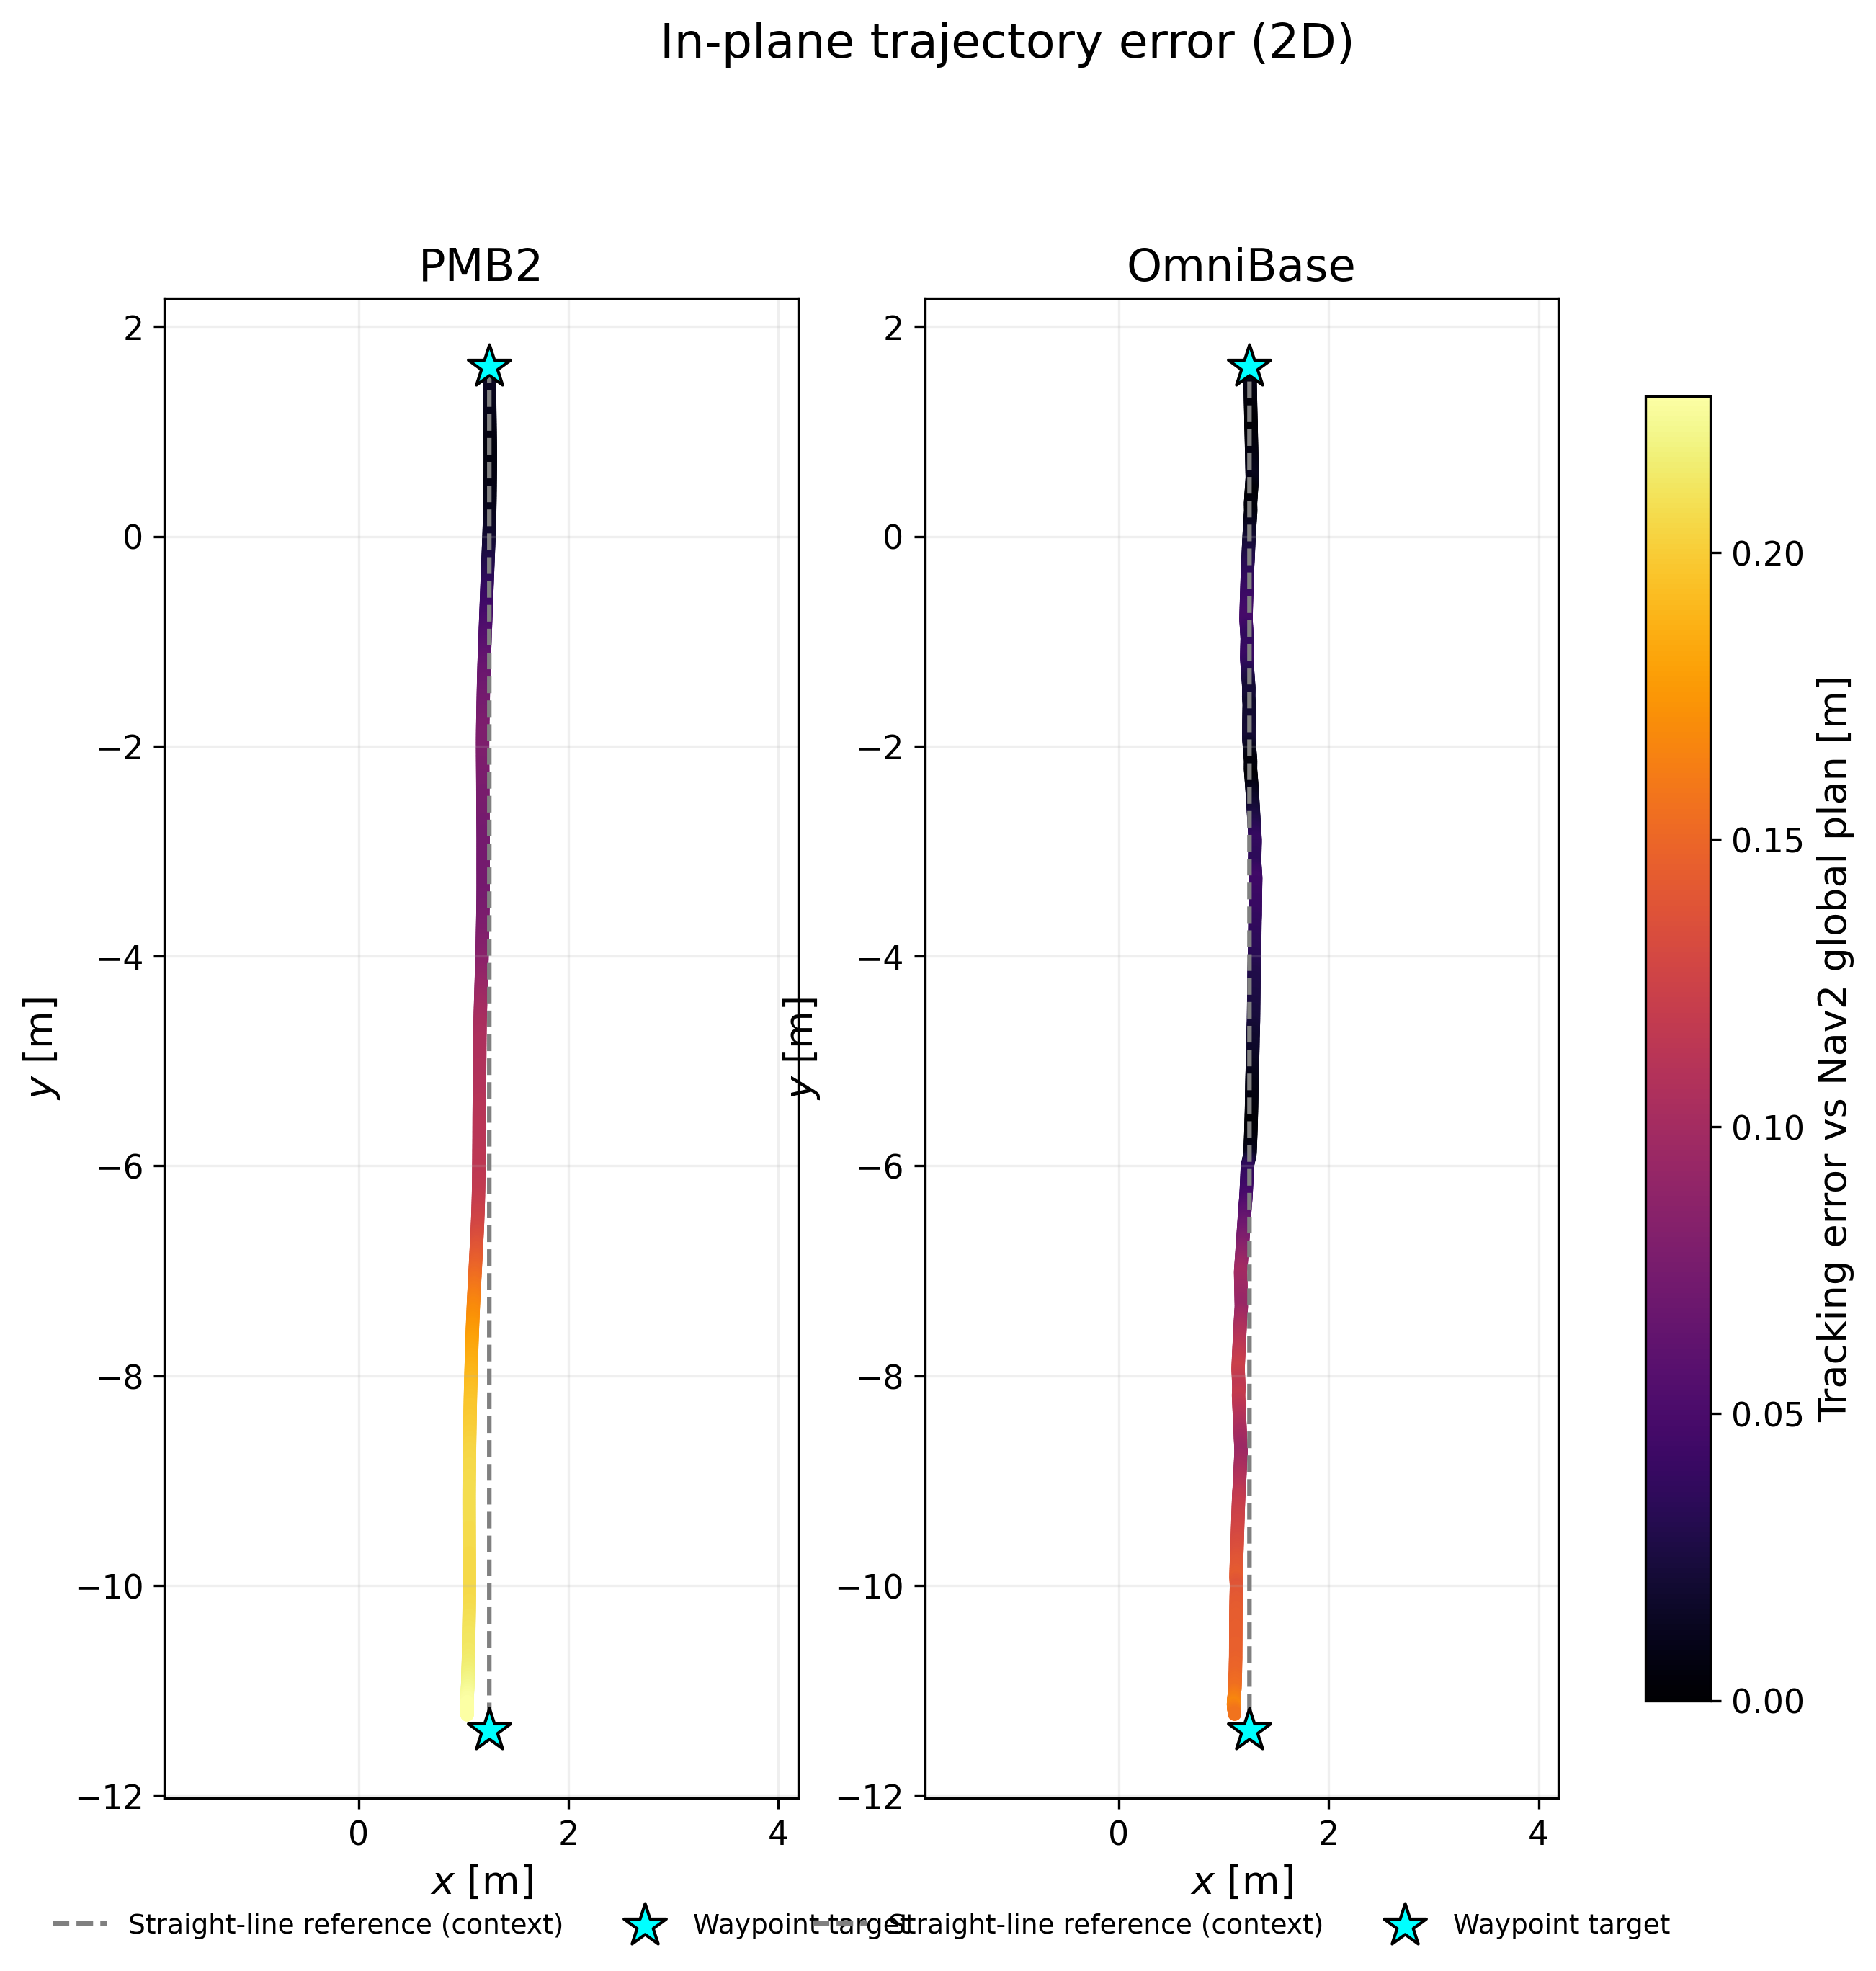
\includegraphics[width=\textwidth]{images/app_B/hallway_cross_track_error_2d.png}
  \caption{Straight corridor: in-plane tracking error (2D). The colour encodes the instantaneous deviation from the Nav2 global plan along the executed trajectory of the median run of each base; the drift accumulates towards the end of the corridor, more markedly for the differential PMB2.}
  \label{fig:app-2d-hallway}
\end{figure}

\begin{figure}[htbp]
  \centering
  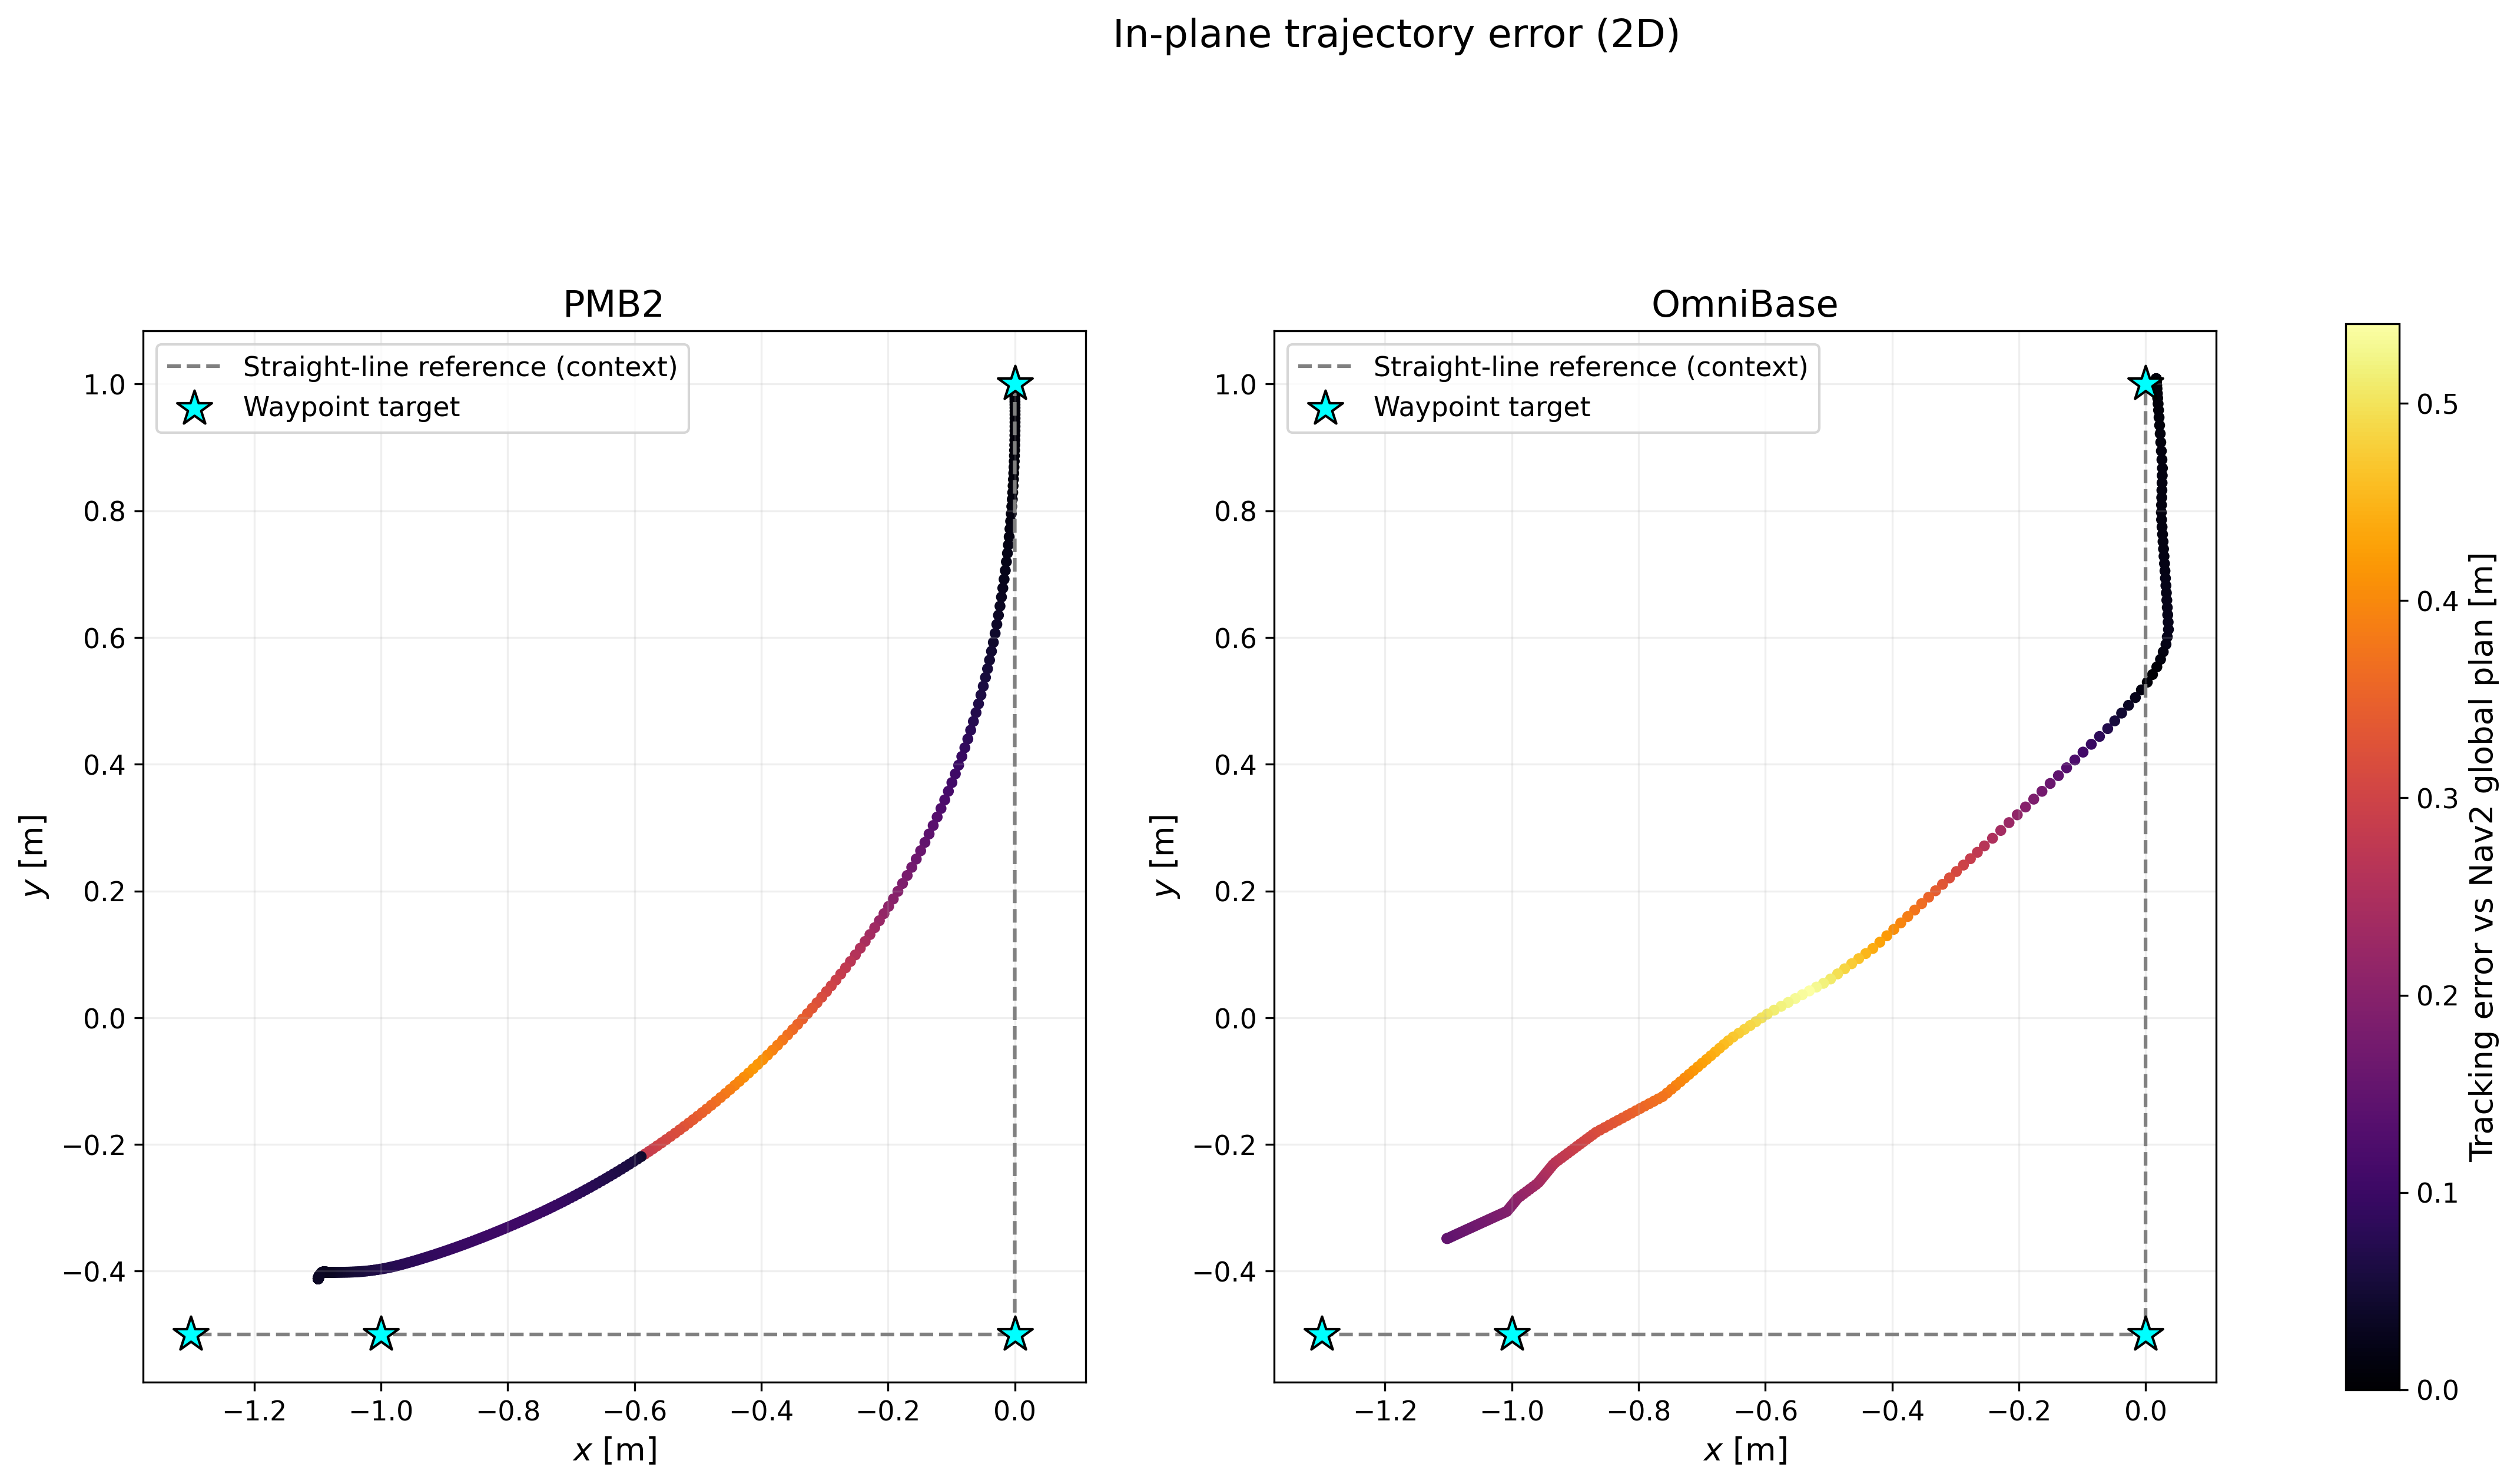
\includegraphics[width=\textwidth]{images/app_B/angle_cross_track_error_2d.png}
  \caption{Sharp corner: in-plane tracking error (2D). The largest deviation from the global plan occurs along the diagonal shortcut of the holonomic OmniBase, consistent with the aggregate values of Section~\ref{subsec:res-angle}.}
  \label{fig:app-2d-angle}
\end{figure}

\begin{figure}[htbp]
  \centering
  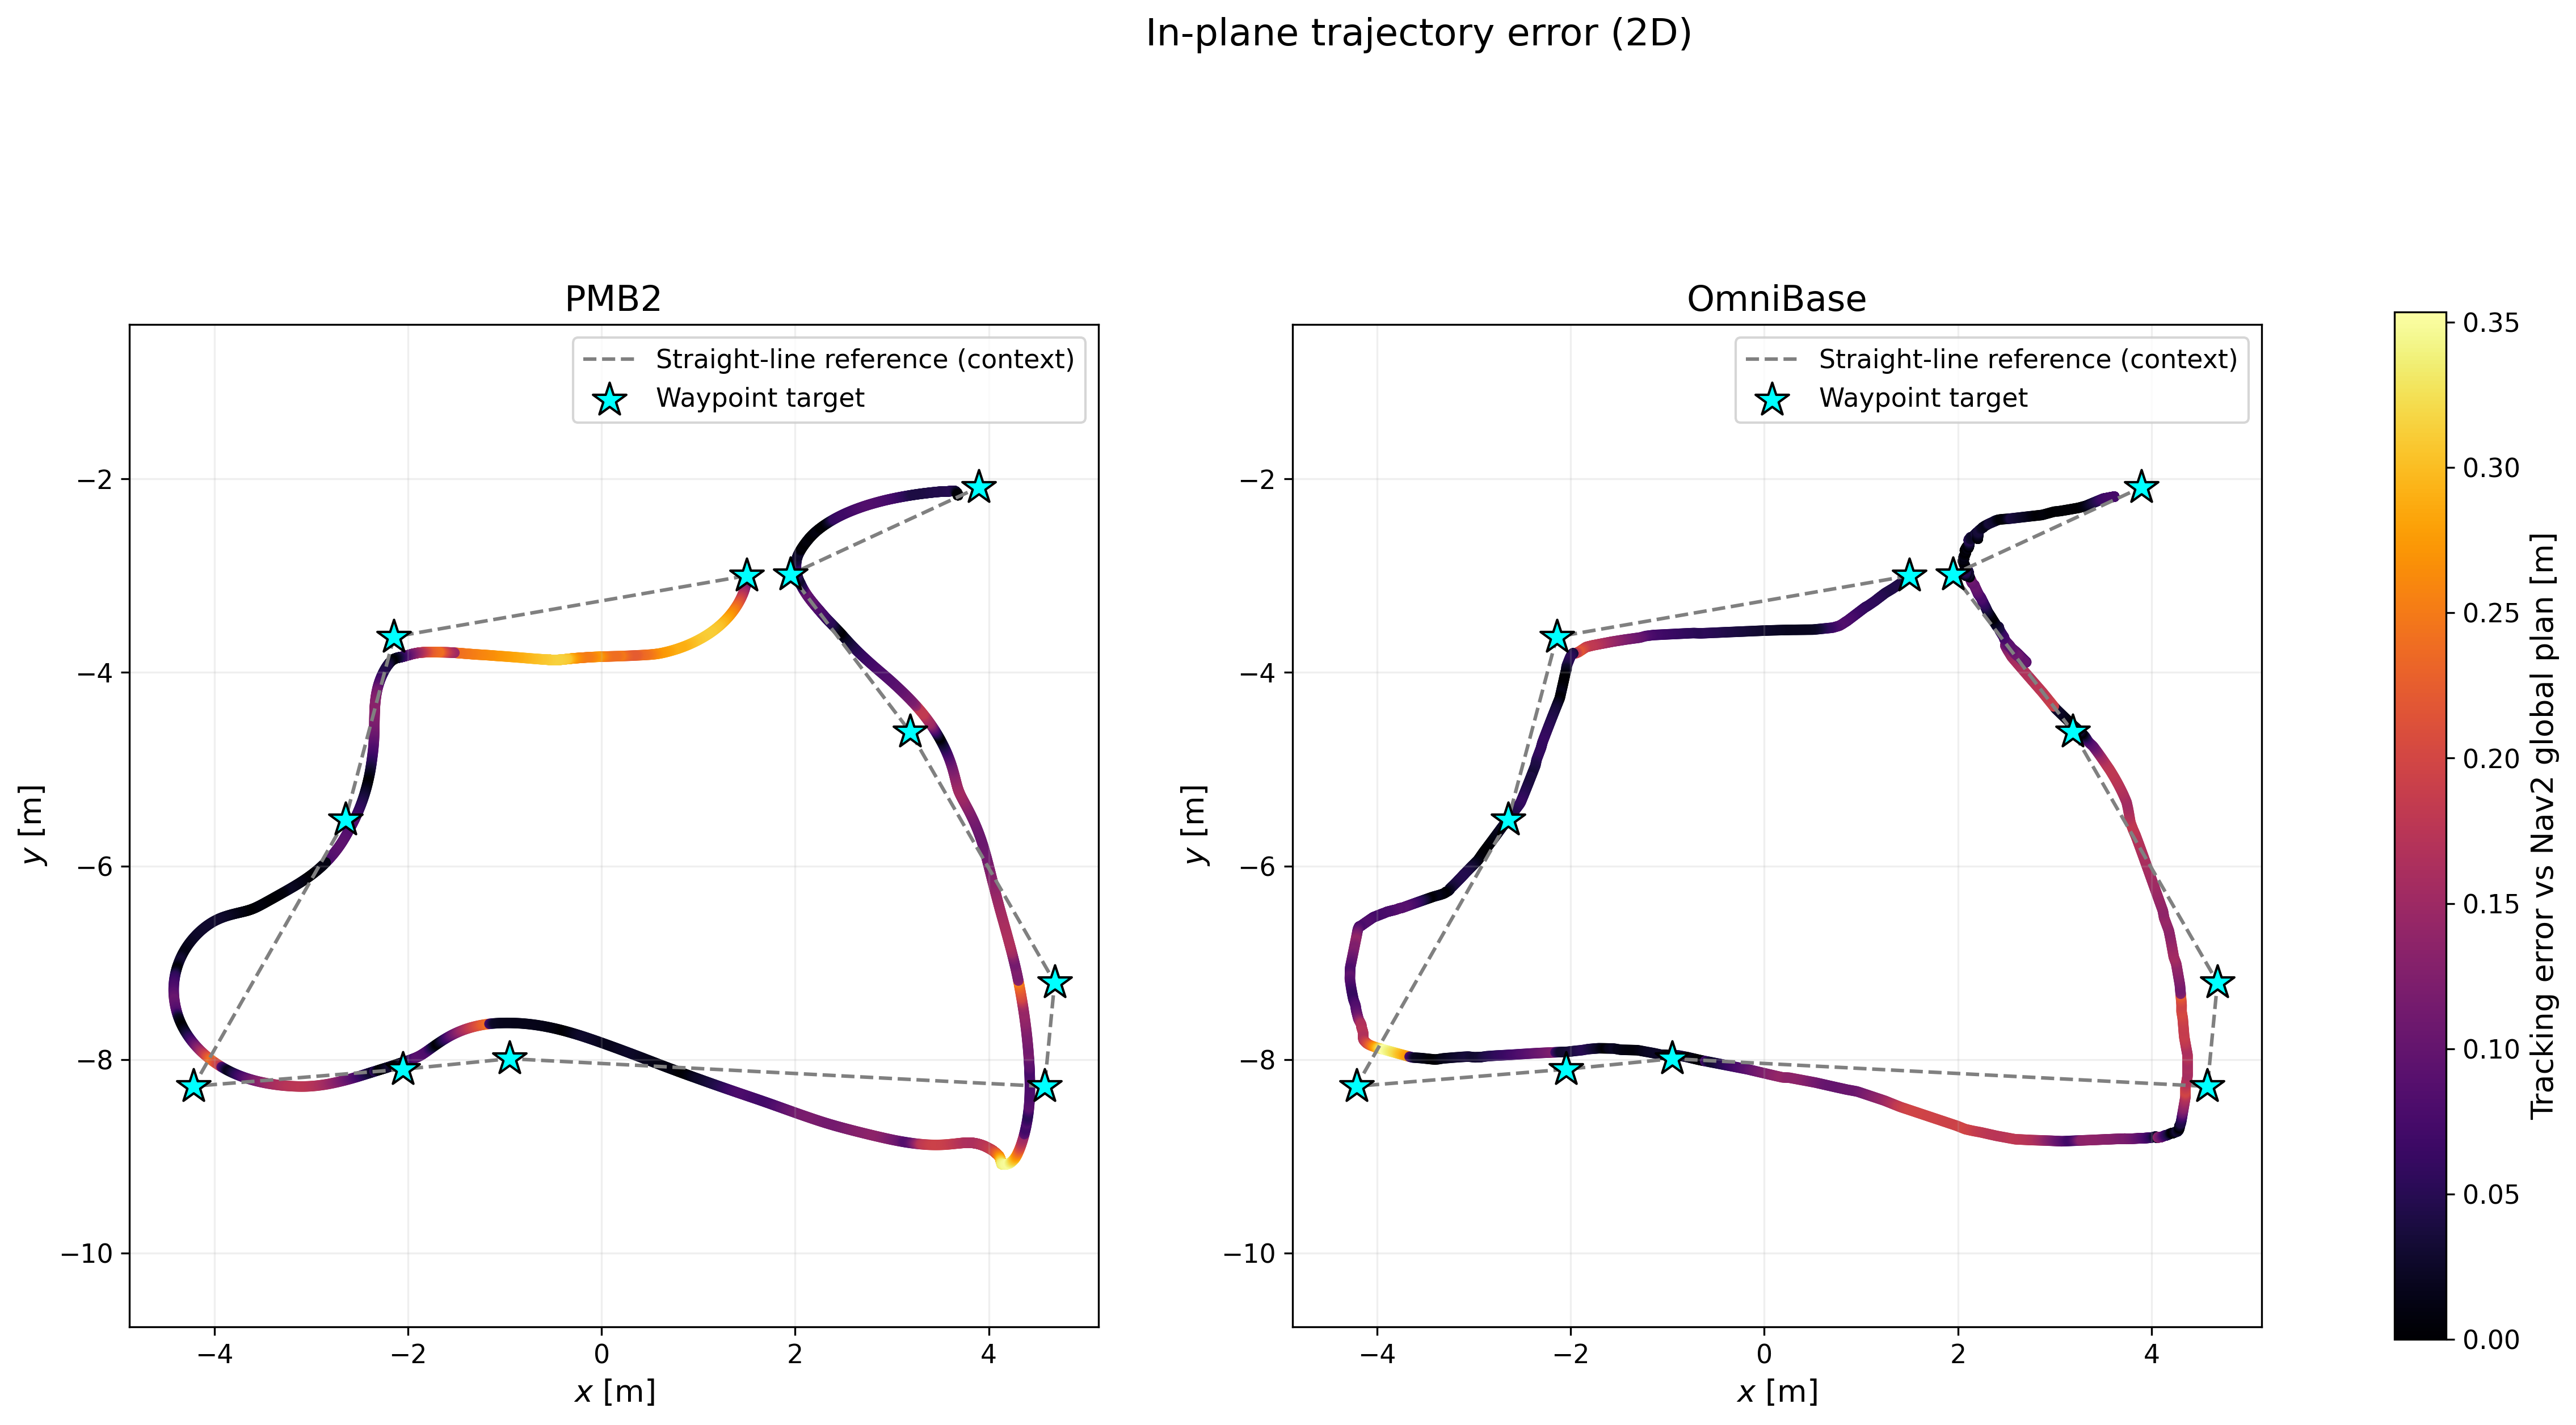
\includegraphics[width=\textwidth]{images/app_B/obs_cross_track_error_2d.png}
  \caption{Cluttered obstacle course: in-plane tracking error (2D). The deviation from the global plan is distributed along the whole circuit and peaks at the tight manoeuvres, remaining lower on average for the holonomic OmniBase.}
  \label{fig:app-2d-obs}
\end{figure}

\begin{figure}[t]
  \centering
  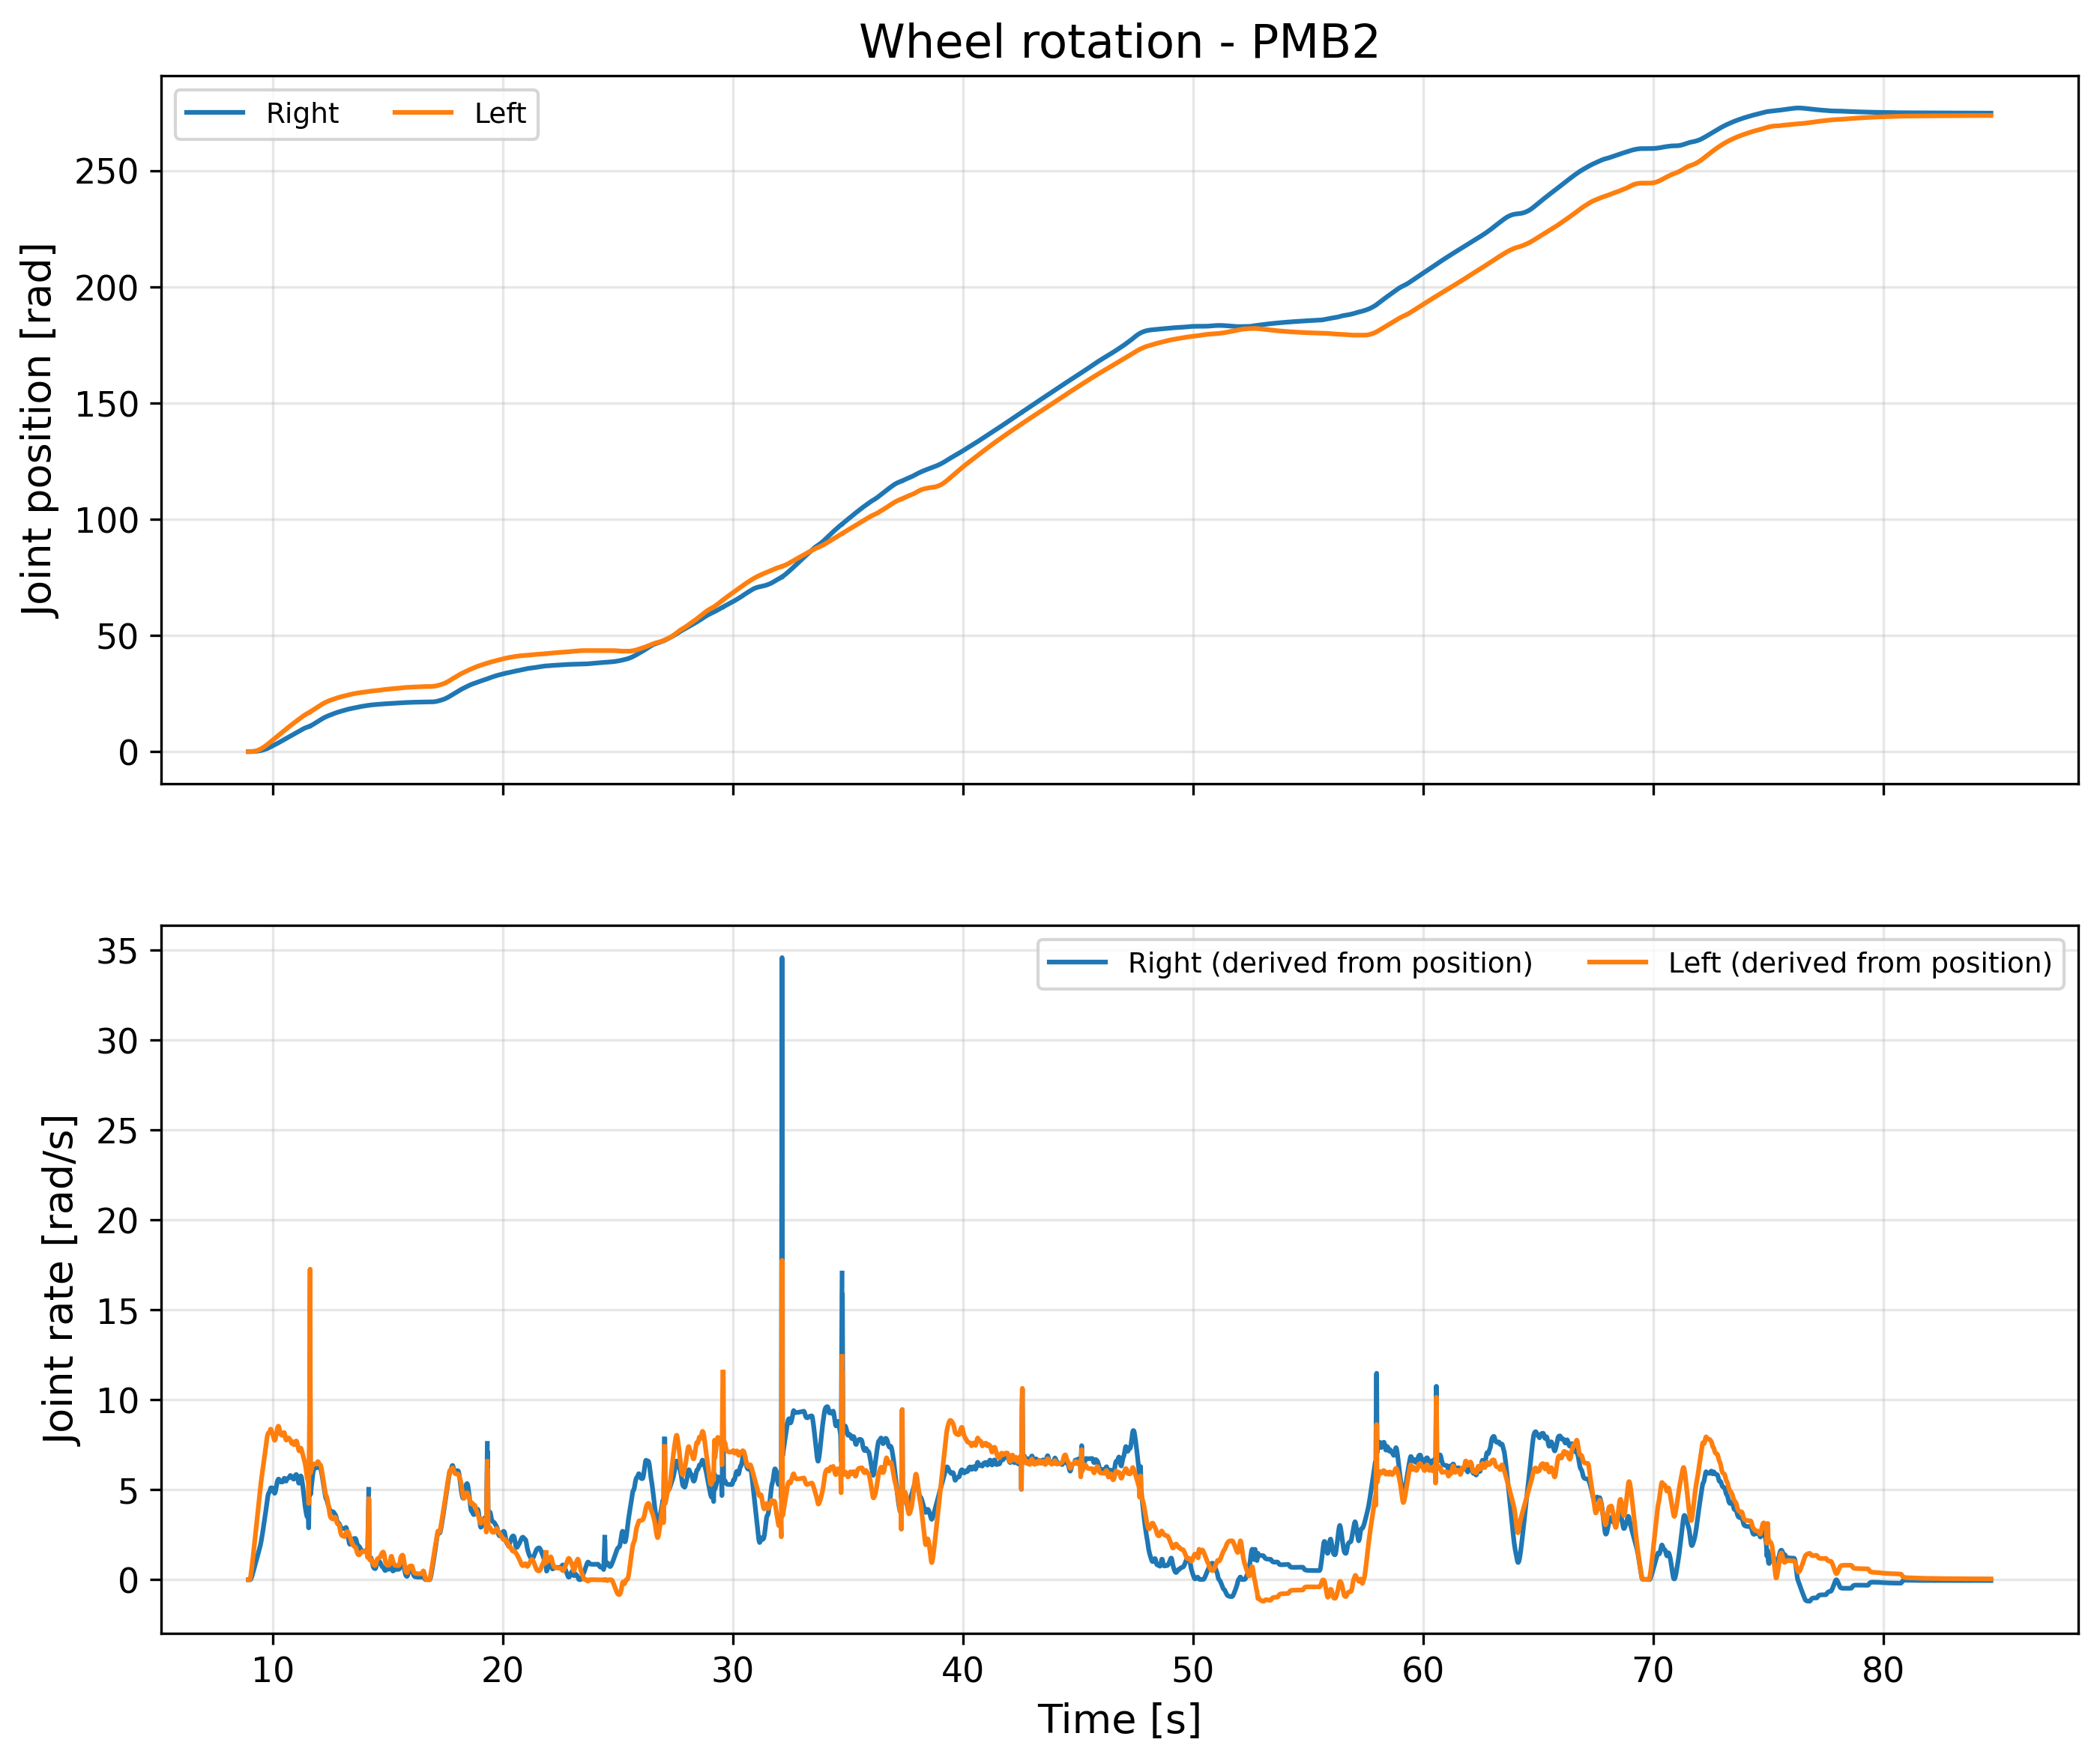
\includegraphics[width=\textwidth]{images/app_B/wheel_rotation_pmb2.png}
  \caption{Cluttered obstacle course: wheel rotation over time for the differential PMB2. In contrast to the straight corridor (Figure~\ref{fig:hallway-wheels-pmb2}), the frequent turns and manoeuvres produce strongly varying, repeatedly reversing wheel rotations.}
  \label{fig:app-wheels-obs-pmb2}
\end{figure}

\begin{figure}[t]
  \centering
  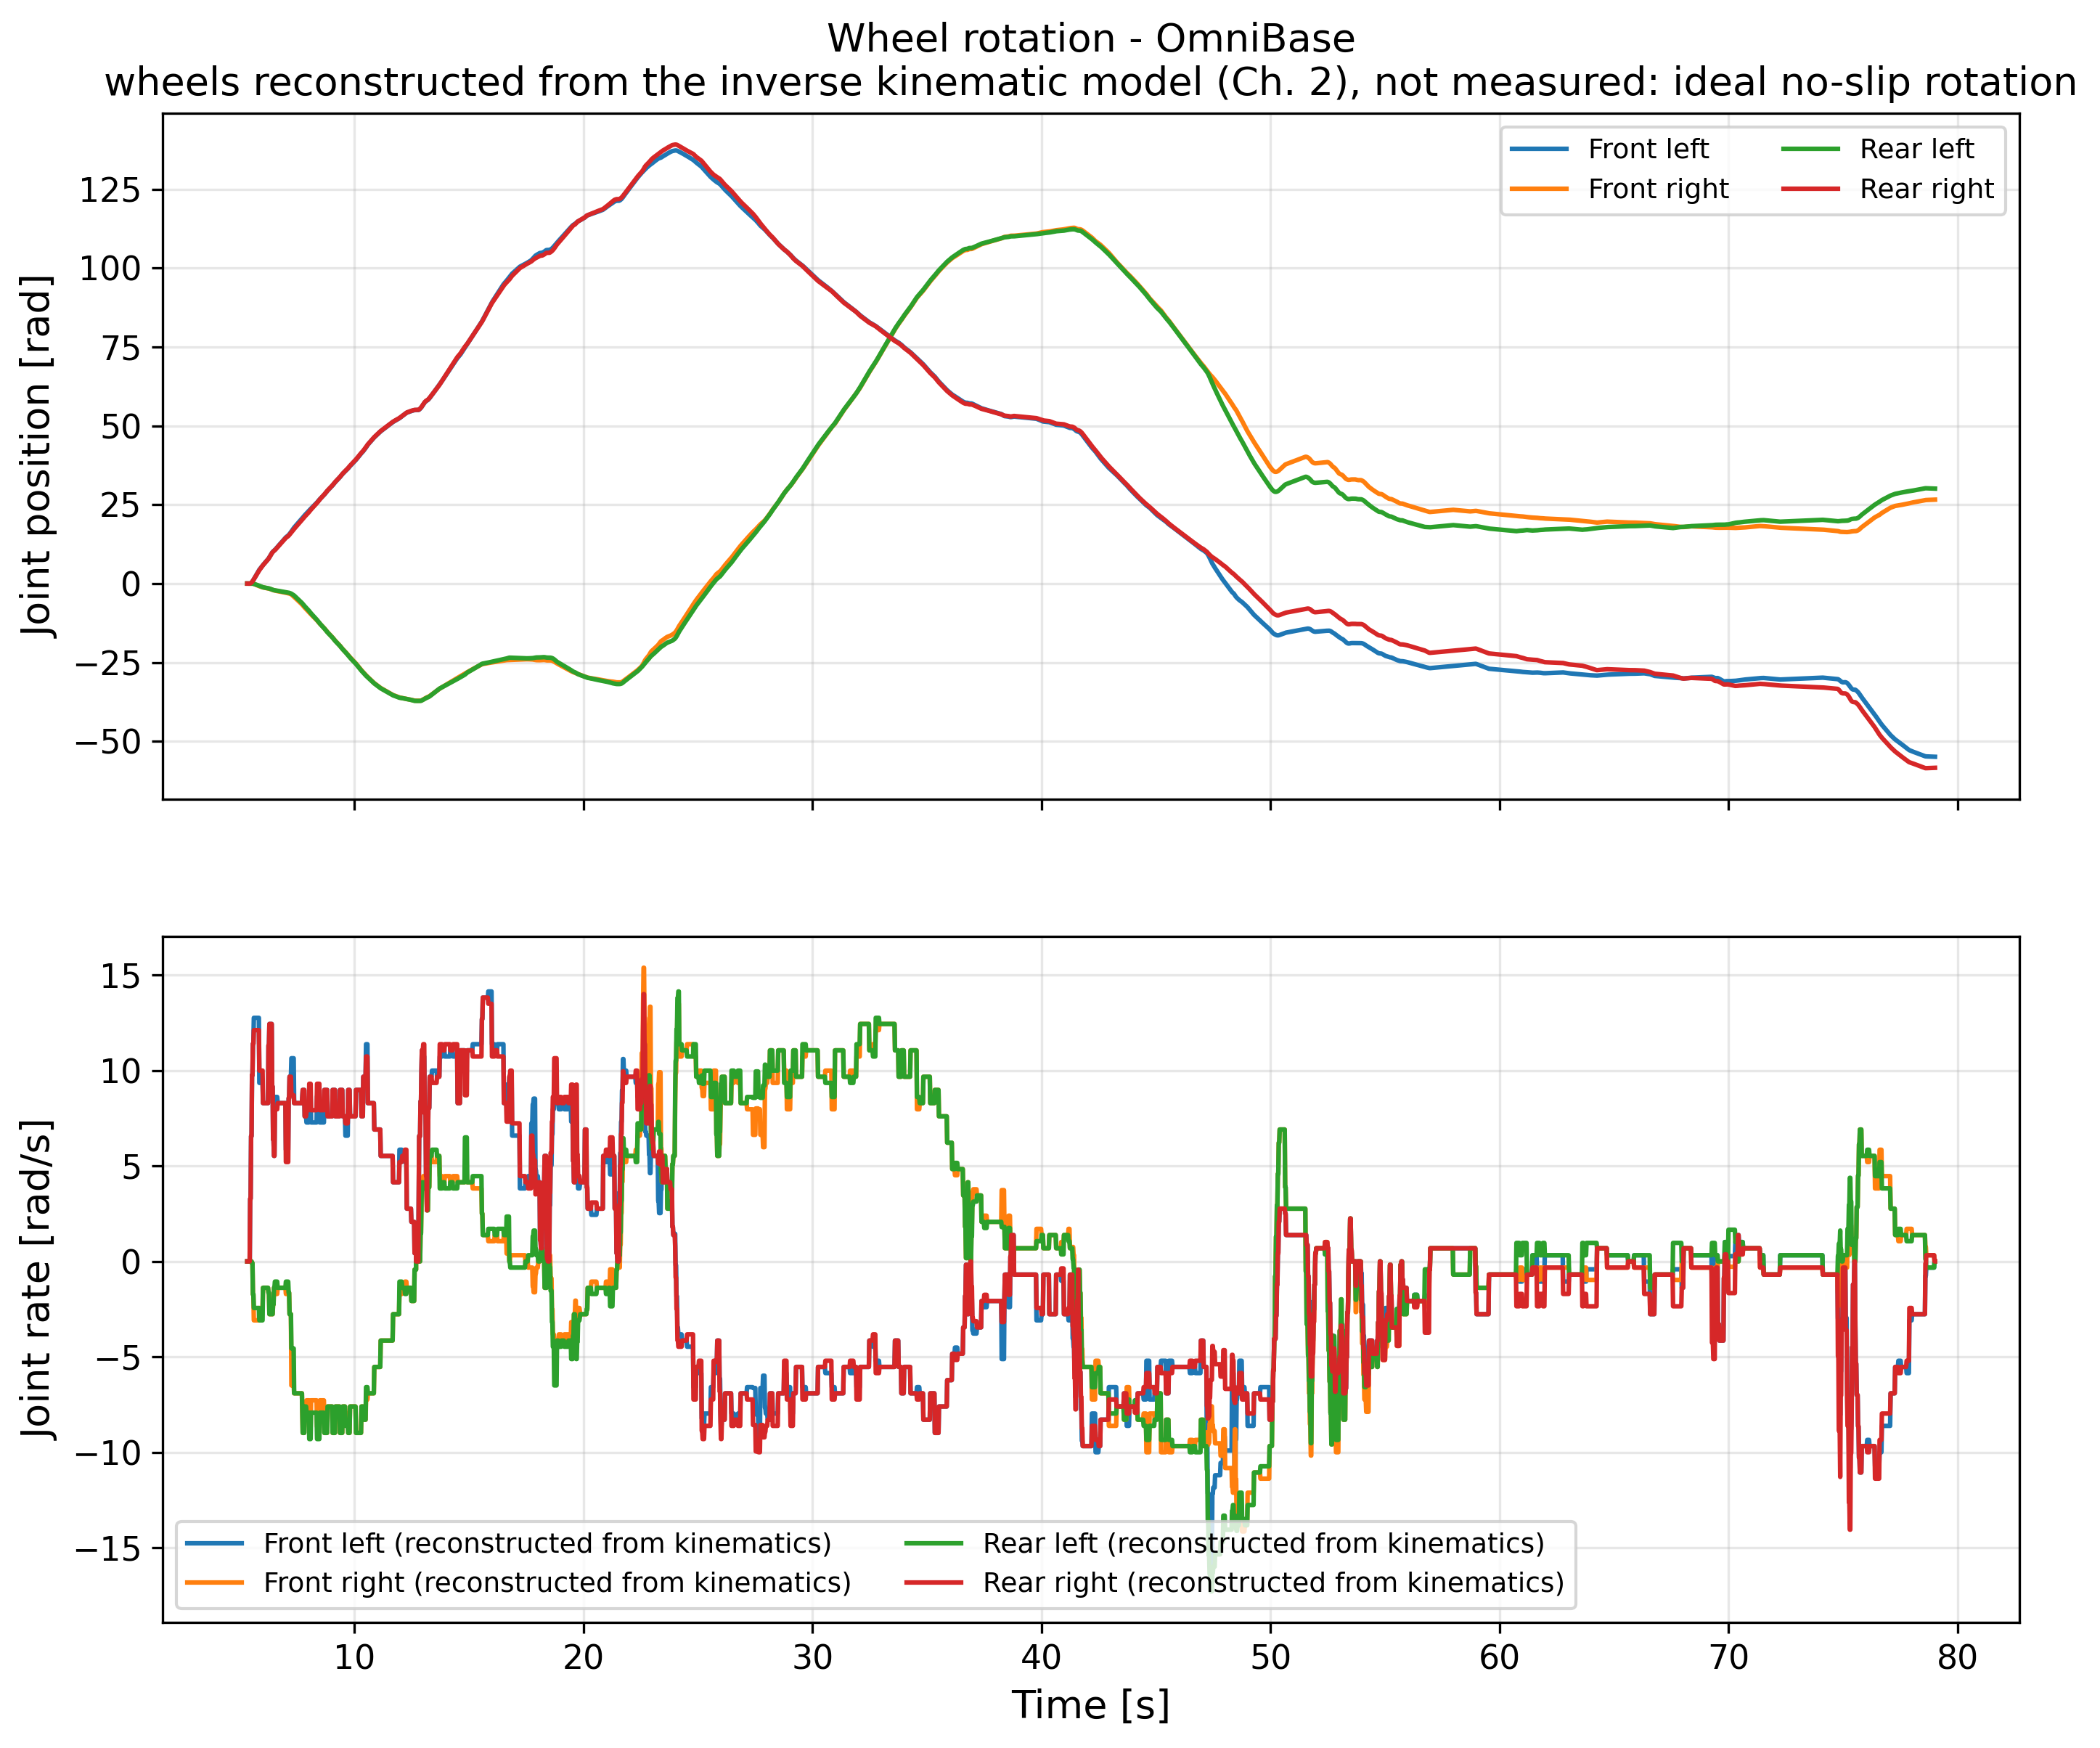
\includegraphics[width=\textwidth]{images/app_B/wheel_rotation_omni.png}
  \caption{Cluttered obstacle course: wheel rotation over time for the holonomic OmniBase, reconstructed from the inverse kinematic model of Chapter~\ref{Ch:Kinematic} (ideal no-slip rotation). The rich, frequently reversing profile reflects the combination of forward and lateral motion used to thread the cluttered circuit.}
  \label{fig:app-wheels-obs-omni}
\end{figure}

\begin{figure}[t!]
  \centering
  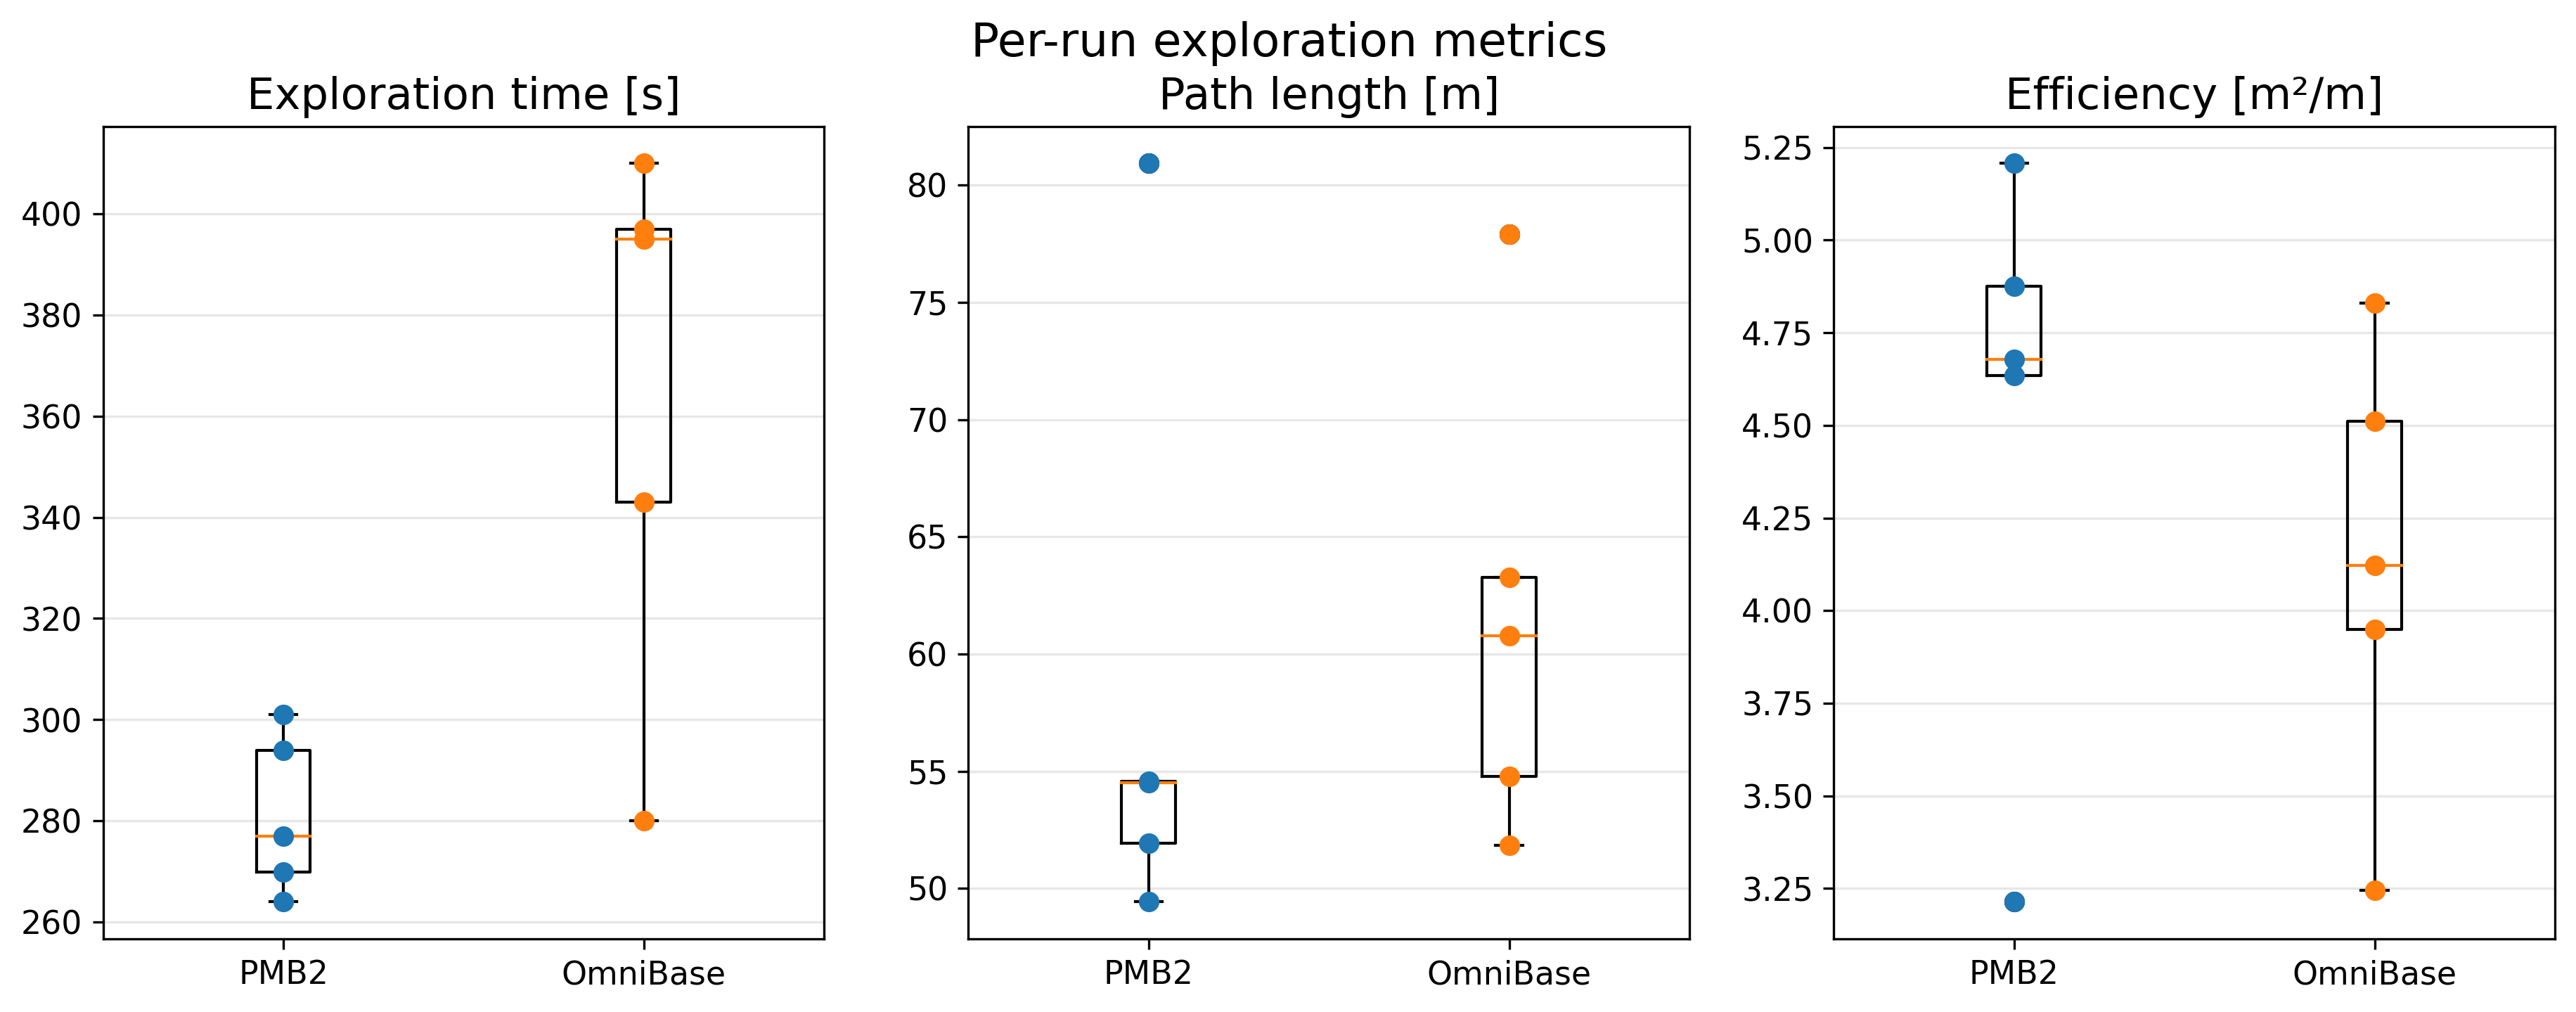
\includegraphics[width=\textwidth]{images/app_B/exploration_metrics_box.png}
  \caption{Autonomous exploration: per-run distribution of exploration time, path length, and area-per-metre efficiency. Complementing the aggregate values of Table~\ref{tab:explore}, the box plots expose the run-to-run spread hidden by the mean: the differential PMB2 is consistently faster and more efficient across its five runs, while the holonomic OmniBase shows a wider spread in both time and efficiency.}
  \label{fig:app-explore-box}
\end{figure}